%%%%%%%%%%%%%%%%%%%%%%%%%%%%%%%%%%%%%%%%%%%%%%%%%%%%%%%%%%%%%%%%%%%%%%%%%%%%%%%%%%%%%%%%%%%%%%%%%%%%%%
% Plantilla básica de Latex en Español.
%
% Autor: Andrés Herrera Poyatos (https://github.com/andreshp)
%
% Es una plantilla básica para redactar documentos. Utiliza el paquete fancyhdr para darle un
% estilo moderno pero serio.
%
% La plantilla se encuentra adaptada al español.
%
%%%%%%%%%%%%%%%%%%%%%%%%%%%%%%%%%%%%%%%%%%%%%%%%%%%%%%%%%%%%%%%%%%%%%%%%%%%%%%%%%%%%%%%%%%%%%%%%%%%%%%

%-----------------------------------------------------------------------------------------------------
%	INCLUSIÓN DE PAQUETES BÁSICOS
%-----------------------------------------------------------------------------------------------------

\documentclass{article}

% Lenguaje
\usepackage[spanish,es-noquoting, es-tabla, es-lcroman]{babel}
\usepackage[utf8]{inputenc}
\selectlanguage{spanish}


% Matemáticas
\usepackage{amsthm}
\usepackage{amsfonts}
\usepackage{amsmath}
\usepackage{tikz-cd}
\theoremstyle{plain}
\newtheorem{theorem}{Teorema}
\newtheorem{proposition}{Proposición}
\newtheorem{lemma}{Lema}
\newtheorem{corollary}{Corolario}
\theoremstyle{definition}
\newtheorem{definition}{Definición}
\theoremstyle{remark}
\newtheorem*{remark}{Nota}
\renewcommand*{\proofname}{Demostración}

% Corrige el espacio previo a las definiciones
\makeatletter
\def\thm@space@setup{%
  \thm@preskip=\parskip \thm@postskip=0pt
}
\makeatother

% Fuente
\usepackage{courier}
\usepackage{microtype}


% ----
% Estilo de página
%----
% Paquetes para el diseño de página:
\usepackage{fancyhdr}               % Utilizado para hacer títulos propios.
\usepackage{lastpage}               % Referencia a la última página. Utilizado para el pie de página.
\usepackage{extramarks}             % Marcas extras. Utilizado en pie de página y cabecera.
\usepackage[parfill]{parskip}       % Crea una nueva línea entre párrafos.
\usepackage{geometry}               % Asigna la "geometría" de las páginas.

% Se elige el estilo fancy y márgenes de 3 centímetros.
\pagestyle{fancy}
\geometry{left=3cm,right=3cm,top=3cm,bottom=3cm,headheight=1cm,headsep=0.5cm} % Márgenes y cabecera.
\fancyhf{}

% Espacios en el documento:
\linespread{1.1}                        % Espacio entre líneas.
\setlength\parindent{0pt}               % Selecciona la indentación para cada inicio de párrafo.

% Cabecera del documento. Se ajusta la línea de la cabecera.
\renewcommand\headrule{
	\begin{minipage}{1\textwidth}
	    \hrule width \hsize
	\end{minipage}
}

% Texto de la cabecera:
\lhead{\docauthor}                          % Parte izquierda.
\chead{}                                    % Centro.
\rhead{\subject \ - \doctitle}              % Parte derecha.

% Pie de página del documento. Se ajusta la línea del pie de página.
\renewcommand\footrule{
\begin{minipage}{1\textwidth}
    \hrule width \hsize
\end{minipage}\par
}

\lfoot{}                                                 % Parte izquierda.
\cfoot{}                                                 % Centro.
\rfoot{Página\ \thepage\ de\ \protect\pageref{LastPage}} % Parte derecha.


% ----
% PORTADA
% ----

% Estilo
\usepackage{title1}

% Título y autores
\newcommand{\doctitle}{Aplicación a gráficos por ordenador}
\newcommand{\docsubtitle}{}
\newcommand{\docdate}{1 \ de \ Enero \ de \ 2015}
\newcommand{\subject}{Cuaternios}
\newcommand{\docauthor}{D. Charte, J.C. Entrena, L. Soto, M. Román}
\newcommand{\docaddress}{Universidad de Granada}
\newcommand{\docemail}{}

% Resumen
\newcommand{\docabstract}{El cálculo de orientaciones en el espacio
  tridimensional es necesario para la generación de gráficos y
  animaciones por ordenador. Los ángulos de Euler representan el
  espacio de orientaciones pero no forman un homeomorfismo local, lo
  que causa errores gráficos (bloqueo del cardán), mientras que los
  cuaterniones de Hamilton sí proporcionan un recubrimiento de dos
  hojas del mismo. Con ellos presentaremos un ejemplo de movimiento de
  objetos en gráficos tridimensionales.}

\begin{document}

\maketitle

% Profundidad del Índice
%\setcounter{tocdepth}{1}
\newpage
\tableofcontents
\newpage

\section{El grupo de rotación}
\subsection{El grupo de rotación SO(3)}

\begin{definition}
  Llamamos $O(n)$ al grupo de las \textbf{matrices ortogonales} reales
  de dimensiones $n \times n$ con la operación de composición; es
  decir,
  \[O(n) = \left\{ M \in GL(n) \mid MM^t=M^tM = I_n \right\}.\]
\end{definition}

Nótese que las matrices ortogonales forman un subgrupo del grupo
lineal $GL(n)$ de matrices invertibles; y que, como consecuencia de la definición, sólo
pueden tener determinante $1$ y $-1$. Las matrices ortogonales dentro
de $GL(n)$ representan las \textit{isometrías} dentro del grupo de isomorfismos.

\begin{definition}
  Llamamos $SO(n)$ al \textbf{subgrupo de rotaciones}, definido como
  el subgrupo de $O(n)$ formado por aquellas matrices que tienen
  determinante $1$. Es decir,
  \[SO(n) = \left\{ M \in O(n) \mid \mathrm{det}(M)=1 \right\}.\]
\end{definition}

En este texto estudiaremos $SO(3)$, las rotaciones de $\mathbb R^3$
dejando fijo el origen, por ser las que pueden aplicarse a la generación
de gráficos tridimensionales por computador. Nuestro interés último
será poder representar las rotaciones de este espacio de forma que
simplifique nuestros cálculos al trabajar con ellas.
Empezaremos estudiando ciertas propiedades del grupo de carácter
geométrico, y pasaremos a otras relacionadas con la topología del
espacio.


\subsection{Ejes de rotación}
En la siguiente proposición demostraremos que cualquier rotación deja
una recta invariante, cuyos puntos se mantienen todos fijos tras
aplicar la rotación. Llamaremos a esta recta el \textbf{eje de rotación}
de la transformación.

\begin{proposition}
  Cada rotación de $SO(3)$ deja fija una recta.
  % TODO: Aquí hay existencia y unicidad, ¿no? Deja fija exactamente a una recta.
\end{proposition}
\begin{proof}
  Sea $ M \in SO(3)$ una rotación. Comprobaremos que la matriz tiene
  al $1$ como valor propio, lo que nos dará un subespacio de al menos
  dimensión 1 cuyos puntos se mantendrán fijos por $M$.

  Que el $1$ sea valor propio equivale a que $\mathrm{det}(M-I_3)=0$.
  Si desarrollamos la expresión sabiendo que $M^t = M^{-1}$ obtenemos
  \[\begin{aligned}
    \mathrm{det}(M - I_3) &=
    \mathrm{det}((M - I_3)^t) \mathrm{det}(M^t - I_3) =
    \mathrm{det}(M^{-1} - I_3) =
    \mathrm{det}(M^{-1}(I_3 - M)) =\\
    &= \mathrm{det}(M^{-1}) \mathrm{det}(I_3 - M) =
    \mathrm{det}(I_3 - M) = -\mathrm{det}(M - I_3),
  \end{aligned}\]
  de donde se deduce directamente que $\mathrm{det}(M - I_3) = 0$ y que el $1$
  es un valor propio de $M$.
\end{proof}

\begin{proposition}
  Cada rotación de $SO(3)$ está determinada de manera única por un
  eje de rotación y un ángulo. Podemos notar así a cada rotación por
  $\mathbf{R}_{\alpha,u}$, donde $\alpha$ es el ángulo de rotación y $u$
  un vector unitario determinando el eje de rotación.
\end{proposition}
\begin{proof}
  Hemos probado anteriormente que cada rotación deja fijo un eje. Si
  proyectamos perpendicularmente a él, nos queda una rotación en el
  plano, que está determinada de forma única por un ángulo. Nótese que
  si existiera otro eje de rotación, debería permanecer fija su
  proyección al plano, pero los giros no triviales en el plano no
  dejan ningún eje fijo.
\end{proof}

\subsection{Propiedades topológicas de las rotaciones}
\begin{proposition}
  El grupo $SO(3)$, con la topología inducida desde la topología usual
  de las matrices, es homeomorfo al espacio proyectivo tridimensional
  $\mathbb{RP}^3$.
\end{proposition}
\begin{proof}
  Consideramos una bola cerrada en $\mathbb R^3$ de radio $\pi$,
  $\mathbb B = \overline{B(0, \pi)}$. Asignamos a cada punto $x \in \mathbb B$
  una rotación, con eje orientado la recta que une el origen y $x$, y ángulo de
  rotación $\alpha = d(x, O)$ la distancia al origen, en el sentido del eje. De
  esta forma, cada punto representa una única rotación, salvo los
  puntos antípoda de la esfera, a los que corresponden las rotaciones de ángulos
  $\pi$ en ambas orientaciones del eje, que son la misma. Esto nos lleva a identificar
  los puntos antípoda de $\partial \mathbb B$, lo que establece un
  homeomorfismo entre $SO(3)$ y $\mathbb{RP}^3$.
\end{proof}


De este resultado se deduce que $SO(3)$ es \textit{conexo} y que tiene un grupo
fundamental no trivial, no siendo, por tanto, \textit{simplemente conexo}.


\section{Ángulos de Euler}
\subsection{Definición}

Se conoce como sistema de los \textbf{ángulos de Euler} al que utiliza
tres ángulos para describir la orientación de un objeto respecto a un
sistema de coordenadas fijo en el espacio. Análogamente, podemos no
considerar como fijo el sistema de coordenadas y ver los ángulos de
Euler como una orientación de dicho sistema. %???

La forma tradicional de usar rotaciones en el espacio se basa en el
uso de las llamadas \textit{rotaciones de Euler}, que combinan hasta tres
rotaciones sobre los ejes cartesianos, donde la única restricción es
que no puede haber dos rotaciones sobre el mismo eje contiguas, pues
derivarían en una. Esas tres rotaciones sobre los ejes cartesianos se
pueden combinar de 12 formas distintas, consistentes en las 6
ordenaciones posibles usando los tres índices, además de aquellas seis
en las que aparece el mismo eje al principio y al final, y uno de los
dos restantes en la posición central. % ¿Qué son exactamente las rotaciones de Euler?

% Faltaría una definición más formal de ángulos de Euler.

\subsection{Descomposición}

% Esto parece un teorema que habría que demostrar
% ¿La unicidad la tenemos?

Cada rotación se descompone en sus tres rotaciones de Euler de forma
única.  En la siguiente fórmula escribimos las matrices de rotación
respecto a los ejes cartesianos, de forma que la primera es la
rotación de ángulo $\psi$ sobre el eje $z$, la segunda rota $\phi$
grados sobre el eje $y$, y la tercera la que rota $\theta$ grados con
respecto al eje $x$. Las tres rotaciones están consideradas en sentido
antihorario.  \footnote{Para cambiar el sentido no hay más que
  cambiarle el signo a los senos}

\[
  \mathbf{R}_{\psi,z}
  \mathbf{R}_{\phi,y}
  \mathbf{R}_{\theta,x} =
  \begin{pmatrix}
    \cos \psi & -\sin \psi & 0 \\
    \sin \psi & \cos \psi & 0 \\
    0 & 0 & 1
  \end{pmatrix}\begin{pmatrix}
      \cos \phi & 0 & \sin \phi \\
      0 & 1 & 0 \\
      -\sin \phi & 0 & \cos \phi
    \end{pmatrix}\begin{pmatrix}
    1 & 0 & 0 \\
    0 & \cos \theta & -\sin \theta \\
    0 & \sin \theta & \cos \theta
  \end{pmatrix}
\]

Podemos ver el espacio de los ángulos de Euler como el 3-toro
$\mathbb T^3$, sin más que identificar cada variable de giro en una
dimensión del toro.

% https://es.wikipedia.org/wiki/Teorema_de_rotaci%C3%B3n_de_Euler

\subsection{Bloqueo del cardán}

El principal problema del uso de los ángulos de Euler es el llamado
\textbf{bloqueo del cardán}. Este fenómeno consiste en la pérdida de
un grado de libertad a la hora de rotar, debida a la alineación de dos
de los ejes de rotación. Esto ocurre naturalmente bajo ciertas
combinaciones en los ángulos de rotación, que provocan que el primero
de los ejes quede alineado con el tercero.

\begin{figure}[ht!]
\centering
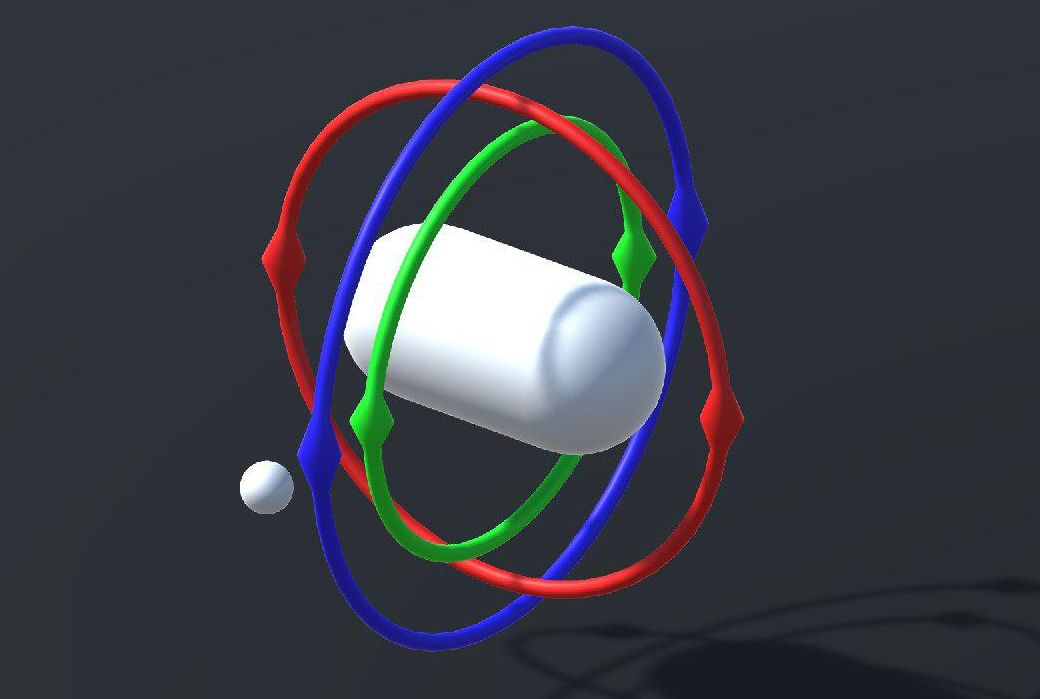
\includegraphics[width=90mm]{cardan.jpg}
\caption{Bloqueo del cardán \label{figcardan}}
\end{figure}

En la \textit{figura \ref{figcardan}} podemos observar un sistema de ángulos
de Euler con tres ejes de rotación, en el que cada eje depende de
todos los ejes superiores a él. En este caso, los ejes \textit{verde} y \textit{azul}
están en posición de bloqueo de cardán, y sólo podrán salir de esa
posición moviendo previamente el eje intermedio \textit{rojo}.

\begin{proposition}
  El bloqueo del cardán es inevitable si se representan rotaciones
  mediante ángulos de Euler. Específicamente, no existen funciones
  recubridoras entre el espacio de ángulos de Euler y el espacio de
  las rotaciones.
\end{proposition}
\begin{proof}
  Formalmente, el bloqueo del cardán ocurre debido a que la función
  que usamos entre el espacio de los ángulos de Euler y las rotaciones
  no es una función sobreyectiva localmente homeomorfismo (un
  recubrimiento), así que demostraremos que el espacio de los ángulos
  de Euler no puede ser recubridor del espacio de rotaciones. Primero
  notaremos que el espacio de los ángulos de Euler, formado por tres
  ángulos, es homeomorfo a $\mathbb T^3$; mientras que el espacio de
  rotaciones hemos podido comprobar anteriormente que es homeomorfo a
  $\mathbb{RP}^3$.

  La imposibilidad de un recubrimiento puede verse fácilmente tomando
  los grupos fundamentales de ambos espacios. Mientras que el grupo
  fundamental del 3-toro es $\pi(\mathbb T^3, x) \simeq \mathbb Z^3$,
  el grupo fundamental del 3-espacio proyectivo es
  $\pi(\mathbb{RP}^3, x) \simeq \mathbb Z_2$. Como el grupo
  fundamental de un recubridor debe ser subgrupo del grupo fundamental
  del espacio reducido, deducimos que no puede existir un
  recubrimiento entre ambos. De hecho, como $\mathbb Z_2$ no tiene subgrupos
  propios, los posibles espacios recubridores deben tener grupo
  fundamental $\mathbb Z_2$ o ser simplemente conexos.
\end{proof}

\section{Cuaternios}
\subsection{Versores}
Sabemos que el álgebra real de los cuaternios puede escribirse como
$\mathbb{H} = \mathbb{R} \oplus V$, donde $V$ es el espacio vectorial
real tridimensional generado por $i,j,k \in \mathbb{H}$, siendo equivalente la
definición
\[
  V = \left\{ v \in \mathbb{H} \mid v^2 < 0 \right\}.
\]
En la siguiente proposición caracterizaremos los \textit{cuaternios unitarios}
vistos desde esa escritura. Los cuaternios unitarios son aquellos de norma
unidad, es decir, aquellos $q \in \mathbb{H}$ que cumplen que
$\|q\| = qq^\ast = 1$. Serán estos cuaternios unitarios los que nos sirvan
posteriormente para calcular rotaciones del espacio tridimensional.

\begin{proposition}
Los cuaternios unitarios, en particular, pueden escribirse como
$\cos \theta + v \sin \theta$, donde $v$ es un vector de norma unidad del
espacio $V$ visto como $\mathbb{R}^3$. A un cuaternio así escrito se le llama
\textbf{versor}.
\end{proposition}
\begin{proof}
  Si tenemos $q = a + bv$ con $v$ unitario, sabemos que $v^2 = - v(-v) = - vv^\ast = -1$.
  Entonces, si $q$ es unitario,
  \[
    1 = qq^\ast = (a+bv)(a-bv) = a^2 + b^2.
  \]
  Con lo que existirá algún $\theta$ para el que $a = \cos \theta$ y $b = \sin \theta$.
\end{proof}

\subsection{Conexión con SU(2)}

% https://en.wikipedia.org/wiki/Rotation_group_SO(3)#Connection_between_SO.283.29_and_SU.282.29

\begin{definition}
  Llamamos $\mathrm{SU}(n)$, al grupo de las \textbf{matrices complejas unitarias} de dimensiones
  $n \times n$ que además tienen determinante $1$. Es decir,
  \[SU(n) = \left\{ M \in U_n(\mathbb{C}) \mid \mathrm{det}(M) = 1 \right\}.\]
\end{definition}

En particular, nos interesaremos por el caso $SU(2)$ porque podemos
verlo como un embebimiento de la esfera tridimensional en
$\mathbb{R}^4$.

\begin{theorem}\label{su2}
  Cada matriz en $SU(2)$ puede escribirse como
  \[\begin{pmatrix}
      a+bi & c+di \\
      -c+di & a-bi
    \end{pmatrix}\]
  donde $a,b,c,d \in \mathbb{R}$ y $a^2+b^2+c^2+d^2 = 1$.
\end{theorem}
\begin{proof}
  Si tomamos $\alpha,\beta,\gamma,\delta \in \mathbb{C}$ formando una matriz unitaria de
  determinante $1$ como
    \[\begin{pmatrix}
      \alpha & \beta \\
      \gamma & \delta
    \end{pmatrix},\]
  tendremos las relaciones siguientes, obtenidas desde la ortogonalidad que exigimos a la matriz
  \[|\alpha|+|\beta| = 1,
    \quad
    \alpha\delta-\beta\gamma = 1,
    \quad
    \alpha\overline{\gamma} + \beta\overline{\delta} = 0,
  \]
  y que se resuelven con $\alpha = \overline{\delta}$ y
  $\beta = -\overline{\gamma}$; mientras que la primera condición
  nos da la condición $a^2+b^2+c^2+d^2 = 1$.
\end{proof}


\subsection{Cuaternios como esfera de dimensión 4}
Si interpretamos los cuaternios como matrices complejas de dimensiones
$2 \times 2$, como
\[
  1 \mapsto \begin{pmatrix} 1 & 0 \\ 0 & 1 \end{pmatrix},\quad
  i \mapsto \begin{pmatrix} i & 0 \\ 0 &-i \end{pmatrix},\quad
  j \mapsto \begin{pmatrix} 0 & 1 \\-1 & 0 \end{pmatrix},\quad
  k \mapsto \begin{pmatrix} 0 & i \\ i & 0 \end{pmatrix},\quad
\]
tenemos que podemos expresar cualquier elemento de $SU(2)$ como
$a + bi + cj + dk$ para $a,b,c,d \in \mathbb{R}$ cumpliendo
$a^2+b^2+c^2+d^2 = 1$. Pero además, dado un cuaternio $a + bi + cj + dk$,
que sea unitario equivale a
\[a^2+b^2+c^2+d^2 = (a+bi+cj+dk)(a-bi-cj-dk) = 1,\]
luego los cuaternios unitarios son los elementos de $SU(2)$.
A su vez, por lo comprobado anteriormente, los elementos de
$SU(2)$ son vectores unitarios de $\mathbb{R}^4$, teniéndose
que $SU(2) \cong S^3$. La aplicación definida
en el teorema \ref{su2} nos da el isomorfismo entre los dos espacios.
\cite{gelfand63}

\subsection{Recubrimiento del grupo de rotaciones}

A diferencia del caso de los ángulos de Euler, los cuaternios unitales
sí son un recubrimiento del espacio de rotaciones $SO(3)$. Esto se
deduce directamente del hecho de que $S^3$ es un recubridor de dos
hojas de $\mathbb{RP}^3$ (de hecho, es su recubridor universal).

Al ser recubridor de dos hojas, tenemos que los cuaternios que se
identifican por la relación de equivalencia de $\mathbb{RP}^3$
representan la misma rotación, pues van al mismo elemento por la
aplicación recubridora. En este caso, son los cuaternios opuestos.


\section{Rotaciones con cuaternios}
\subsection{Fórmulas de Rodrigues}
Las \textbf{fórmulas de Rodrigues} representan una solución explícita
a la composición de dos rotaciones en el espacio tridimensional sobre
dos vectores distintos y para el cálculo de una rotación sobre un
vector.

\begin{theorem}
  \textbf{Fórmula de Rodrigues para la rotación.} Si llamamos
  $\mathbf{R}_{\alpha,u}$ a la rotación de ángulo $\alpha$ sobre el
  eje dado por un vector no nulo $u$, la rotación de un vector
  $v \in\mathbb{R}^3$ se calcula como
  \[\mathbf{R_{\alpha,u}}v = v \cos \alpha + (u \times v)\sin \alpha + u(u\cdot v)(1-\cos\alpha).\]
\end{theorem}
\begin{proof}
  El vector $v$ podemos descomponerlo en su componente paralela y su
  componente perpendicular a $u$, dadas respectivamente por
  \[w_1 = (v \cdot u) v \quad \text{ y } \quad w_2 = u \times (u \times v).\]
  Nótese que la rotación sólo necesitamos aplicarla a
  la componente perpendicular. Si calculamos la rotación de la
  componente perpendicular tenemos que
  $\mathbf{R_{\alpha,u}} w_2 = \cos(\alpha) w_2 + \sin(\alpha) u \times v$, con
  lo que podemos sustituir en la descomposición $v = w_1+w_2$ para
  tener
  \[\mathbf{R_{\alpha,u}}v =
    w_1 + (v-w_1)\cos\alpha + (u \times v)\sin\alpha =
    v\cos\alpha + (1-\cos \alpha)(u \cdot v)v + (u \times v)\sin\alpha.
  \]
  % https://en.wikipedia.org/wiki/Rodrigues%27_rotation_formula#Derivation
\end{proof}

\begin{theorem}
  \textbf{Fórmula de Rodrigues para la composición.} Si llamamos
  $\mathbf{R}_{\alpha,a}$ a la rotación de ángulo $\alpha$ sobre el
  eje dado por un vector no nulo $a$, la ecuación
  \[\mathbf{R}_{\gamma,c} =\mathbf{R}_{\alpha,a}\mathbf{R}_{\beta,b}\]
  tiene una solución con
  \[\begin{aligned}
    \cos \frac{\gamma}{2} &=
    \cos \frac{\alpha}{2} \cos\frac{\beta}{2} - \sin\frac{\alpha}{2}\sin\frac{\beta}{2} (a\cdot b)\\
    c \sin \frac{\gamma}{2} &=
    \sin \frac{\alpha}{2} \cos\frac{\beta}{2} a +
    \cos \frac{\alpha}{2} \sin\frac{\beta}{2} b +
    \sin \frac{\alpha}{2} \sin\frac{\beta}{2} (a \times b)
  \end{aligned}\]
  donde notamos el producto escalar como $a\cdot b$ y el producto vectorial como $a \times b$.
  \cite{vince11}
\end{theorem}

Es interesante notar entonces cómo el producto de dos \textit{versores}
satisface esta misma fórmula, lo que hará que la multiplicación de
cuaternios pueda ser luego interpretada como la composición de
rotaciones.

Sean los versores dados por
\[
  q_a = \cos \frac{\alpha}{2}  + a \sin \frac{\alpha}{2} ,
  \qquad
  q_b = \cos \frac{\beta}{2} + b \sin \frac{\beta}{2},
  \qquad
  q_c = \cos \frac{\gamma}{2}  + c \sin \frac{\gamma}{2} .
\]
entonces el desarrollo del producto acaba resultando en la fórmula de
Rodrigues con la misma solución
\[\begin{aligned}
    \cos \frac{\gamma}{2} &=
    \cos \frac{\alpha}{2} \cos\frac{1}{2}\beta - \sin\frac{1}{2}\alpha\sin\frac{\beta}{2} (a\cdot b)\\
    c\sin \frac{\gamma}{2} &=
    \sin \frac{\alpha}{2} \cos\frac{\beta}{2} a +
    \cos \frac{\alpha}{2} \sin\frac{\beta}{2} b +
    \sin \frac{\alpha}{2} \sin\frac{\beta}{2} (a \times b).
  \end{aligned}\]

\subsection{Rotación con cuaternios}
Vamos a resolver el problema de cómo rotar un vector del espacio
$V \cong \mathbb{R}^3$ usando cuaternios. La rotación que intentaremos
resolver será de ángulo $\alpha$ y tendrá como eje de rotación el dado
por el vector unitario $u$. Comprobaremos que para rotar un vector $p$
habrá que tomar el cuaternio
\[q = \cos \frac{\alpha}{2} + u \sin \frac{\alpha}{2}\]
y conjugar el vector sobre él, como $R_{\alpha,u}(p) = qpq^\ast $.

\begin{proposition}
Dado un vector $p$, la rotación de ángulo $\alpha$ con el eje dado por
el vector unitario $u$ es
\[ \mathbf{R}_{\alpha,u}p =
  \left(\cos \frac{\alpha}{2} + u \sin \frac{\alpha}{2}\right)
  p
  \left(\cos \frac{\alpha}{2} - u \sin \frac{\alpha}{2}\right).\]
O, si la escribimos tomando un cuaternio unitario
\[
  q = \cos \frac{\alpha}{2} + u \sin \frac{\alpha}{2},
\]
tenemos que $\mathbf{R}_{\alpha,u}p = qpq^\ast $.
\end{proposition}
\begin{proof}
  Simplemente desarrollando
  \[\begin{aligned}
      qpq^\ast &=
      p \cos^2\frac{\alpha}{2} + (up-pu)\sin\frac{\alpha}{2}\cos\frac{\alpha}{2} - upu\sin\frac{\alpha}{2}
      \\&=
      p \left(\cos^2\frac{\alpha}{2} - \sin^2\frac{\alpha}{2} \right) +
      (p \times u)\left(2\sin\frac{\alpha}{2}\cos\frac{\alpha}{2}\right) +
      u(u\cdot p)\left(2\sin^2\frac{\alpha}{2}\right)
      \\&=
      p \cos\alpha +
      (p \times u)\sin\alpha +
      u(u\cdot p)\left(1 - \cos \alpha\right),
    \end{aligned}\]
  que vuelve a ser la fórmula de Rodrigues para la rotación.
\end{proof}

\section{Aplicación en gráficos}

\subsection{Exponenciación de cuaternios}
\begin{definition}
  Se define la función \textbf{exponencial en cuaternios},
  $\exp \colon \mathbb{H} \to \mathbb{H}$, desde la serie de potencias
  de la función exponencial usual, es decir,
  \[\exp(q) =  1 + q + \frac{q^2}{2!} + \frac{q^3}{3!} + \dots + \frac{q^n}{n!} + \cdots\ .
  \]
\end{definition}

Si escribimos los cuaternios como versores,
$q = \cos \theta + v \sin \theta$, tendremos que, como $v^2 = -1$, se
cumple la fórmula de Euler para cualquier $\theta \in \mathbb{R}$ como
$\exp(\theta v) = \cos \theta + v \sin \theta = q$, y por tanto
podemos calcular la exponencial de un cuaternio como
\[q^t = \exp(t \theta v) = \cos (t \theta) + v \sin (t \theta).\]

\subsection{Spherical Linear Interpolation (SLERP)}

El método \textbf{Spherical Lineal Iterpolation (SLERP)} permite
interpolar un punto entre dos orientaciones de manera continua. Dadas
dos orientaciones $q_1,q_2$ representadas como cuaterniones, un punto
$p$ y un parámetro de interpolación $t$, buscamos un camino continuo
que interpole $p$ desde $q_1$, cuando $t=0$, hasta $q_2$, cuando
$t=1$.

Para calcular la rotación interpolada, usamos la fórmula \cite{vince11}
\[q' = q_1(q_1^{-1}q_2)^t \qquad\text{ para } t \in [0,1].\]

Cuando interpolamos usando SLERP, la interpolación de cuaternios
induce a su vez una interpolación en las rotaciones tridimensionales,
que nos dará una rotación con velocidad angular uniforme y alrededor
de un eje fijo.
% Por qué? https://en.wikipedia.org/wiki/Slerp#Quaternion_Slerp

Sin embargo, como el recubrimiento es doble, el camino de rotaciones
puede ser doble y ser o bien el camino más corto, o bien el camino más
largo.

% http://number-none.com/product/Understanding%20Slerp,%20Then%20Not%20Using%20It/
% https://www.geometrictools.com/Documentation/Quaternions.pdf

\subsection{Spherical and Quadrangle (SQUAD)}

El método \textbf{Spherical and Quadrangle (SQUAD)} es un método
similar al método de De Casteljau para el cálculo de curvas de Bézier,
y proporciona una interpolación cúbica entre dos orientaciones
parametrizada por otras dos.

\begin{definition}
Sean $a,b,p,q$ cuatro cuaternios, vistos como vértices entre los que
realizaremos la interpolación cúbica. La idea es interpolar un punto
$c$ entre $p$ y $q$ mientras que, a la vez, interpolamos un $d$ entre
$a$ y $b$; finalmente, interpolamos con una fórmula cuadrática entre
los puntos de las interpolaciones previas $d$ y $c$. Definimos la
interpolación Squad como
\[
  \mathrm{Squad}(p,q,a,b;t) =
  \mathrm{Slerp}(\mathrm{Slerp}(p,q;t), \mathrm{Slerp}(a,b;t); 2t(1-t)).
\]
\end{definition}
% http://run.usc.edu/cs520-s13/assign2/p245-shoemake.pdf

\section{Referencias}
% https://en.wikipedia.org/wiki/Euler_angles
% https://en.wikipedia.org/wiki/Gimbal_lock
% https://en.wikipedia.org/wiki/Rotation_group_SO(3)
% https://en.wikipedia.org/wiki/Plate_trick
% https://en.wikipedia.org/wiki/Charts_on_SO(3)
% https://www.3dgep.com/understanding-quaternions/

\begin{thebibliography}{9}

\bibitem{gelfand63}
  Gelfand, I.M.; Minlos, R.A.; Shapiro, Z.Ya. (1963),
  Representations of the Rotation and Lorentz Groups and their Applications,
  New York: Pergamon Press.

\bibitem{vince11}
  John Vince (2011),
  Quaternions for Computer Graphics,
  Springer-Verlag London.

\end{thebibliography}

\end{document}
